% !TeX document-id = {e96318ba-ee8c-4009-b5ac-484871d58952}
% !TeX encoding = UTF-8
% !TeX program = pdflatex
% !BIB program = bibtex

%%% Um einen Artikel auf deutsch zu schreiben, genügt es die Klasse ohne
%%% Parameter zu laden.
\documentclass[english]{lni}
%%% To write an article in English, please use the option ``english'' in order
%%% to get the correct hyphenation patterns and terms.
%%% \documentclass[english]{class}
%%

\usepackage{subcaption}
\usepackage{tikz}
\usepackage{subcaption}
\usepackage{float}
\usepackage{verbatim}
\begin{document}

\title[Simulating Recognition of Weeds Using Camera-Mounted Drones with Deep Learning]{Simulating Recognition of Weeds Using Camera-Mounted Drones with Deep Learning}
\author[Group 1]{Luca Brodo\footnote{ \email{luca.brodo@stud.hshl.de}}, Niklas Kohlhage\footnote{ \email{niklas.kohlhage@stud.hshl.de}}, Carl-Georg Meyer\footnote{ \email{carl-georg.meyer@stud.hshl.de}}, Jonas Weißbrod\footnote{ \email{jonas.weissbrod@stud.hshl.de}} }
\startpage{1} % Beginn der Seitenzählung für diesen Beitrag / Start page
\booktitle{Autonomous Systems B Lab} % Name of book title
\year{Winter Term 2021}

\maketitle
\tableofcontents
\begin{abstract}
Agriculture has already been around for longer than most people could possibly imagine. The field was revolutionized multiple times over the years, first with animals being introduced to simplify farming processes before being revolutionized again with the help of machines. The next revolution is imminent: the combination of modern unmanned aerial vehicles and deep learning algorithms. The topic is of special interest for farmers, as partly or even fully automated farming systems could have an immense impact on the lives of them and their families. However, it is questionable how difficult a real world application might be and whether farming automation is an option for the near future.
\end{abstract}

\newpage

\section{Motivation}

Automation is becoming ever more present in our culture and extending beyond just factories, constantly evolving. With innovations like self-driving cars, it is becoming part of our personal lives.\\ 
With drones coming in a wide range of price ranges \cite{statistica}, it is easier than ever to apply them to a wide array of applications. In our case this is to help farmers survey their plants with drones, working as a swarm, detect them and collect that information.
This is made easy with what drones are able to do in their current state. They can be small, fast to deploy and are capable of operating at low altitudes \cite{efforg}, all characteristics that help tremendously when being applied to farming. In addition to that, drones are commonly equipped with cameras, another crucial part of equipment that enables us to realise our core idea.\\
Furthermore with our vision, we want to make an impact not just technological wise, but also on the environment. In our collective minds it is the general end-goal to use this project as a way to outline the technical challenges that we are currently facing, how we are overcoming them and how they could be used as a stepping stone for farmers, to make their lives easier whilst supplying an energy friendly solution. This would result in an efficient way for farmers to check up on their fields, enabling them to save my money by being able to other task, saving time as a result.\\
All of this is impossible to realise without deep learning. This is a fairly new technology with it the first computer implementation being achieved as recent as 2006. One definition for deep learning could be "DL is a set of machine learning algorithms that attempt to learn in multiple levels, corresponding to different levels of abstraction"\cite{info10040122}. It is important to note that deep learning applications require a high amount of computational power, which can be supplied by graphics processing units (GPUs). This is needed to have the algorithm train within a reasonable time-frame, which is not achieve able with central processing units (CPUs) due to their lack of memory bandwidth, data-set-size and optimization \cite{info10040122}\cite{runai}.\\
With all that being said, our documentation will initially lay out the approach we went with and follow this up by talking about the models that we created. In addition to that their validation will also be elaborated on. Following that, we illustrate how the data-set was created and the thought process behind it, with visual images of the data-set itself being given. This also includes how the data was collected and augmented. Lastly we lay out our simulation and how we go about plant recognition and the simulation environment.
\newpage

\section[Approach]{Approach\protect\footnote{ \email{jonas.weissbrod@stud.hshl.de}}}\label{sec:approach}

In the beginning it will be talked about, how we approached developing an appropriate solution to the task given to us. Before even considering the principles of model creation, we began to conceptualize the general understanding of what our project is supposed to achieve and what the basic parameter conditions are.\\
This early conceptualization lead to the following theoretical ideas on how the project's parameters could be defined going into the further development. We thought of a prior declaration of the field to mark out the borders of the area that needs to be considered during the workflow. Then, this agricultural area would be divided into multiple squares of same size to enable a more detailed localization capability of the targeted area, with regard to a theoretical rule of thumb, the more square divisions, the more precise the localization. This finishes our consideration of the target area and leaves the aspects of drones and plants open.\\
Coming to the thoughts about the plants and their handling, with processes that could exceed the projects limits. From our point of view there are two different types of vegetation on the field, with the consciously planted crops and the weed that grows by its own, which can be considered as unwanted. Therefore, we also thought of the possibility of using fertilizers to sustain the planted crops and herbicides to avoid or decrease the amount of weed on the field. Those ideas continued with the model creation, but were dropped afterwards to focus on the important aspects of the task.\\
The last concept that was regarded by us in the first concepts was the role of the drones in the overall system. We came up with the understanding that there will be multiple drones used in the workflow and therefore we require a controlling element. This was decided to be the role of the \textit{control room}, that observes the operation and controls the drones, with providing target areas and task allocation. Following, the drones will administer most of the tasks necessary prepare an agricultural area, beside the active planting and harvesting of the crops. Those tasks mainly include the applied observation of the field and the distribution of fertilizers and herbicides. With the considerations of the field, the plant and the drones covered, the first conceptualization is complete and will be followed by two use cases and one activity diagram as examples, to explain the process of model creation.

\subsection{Use case diagram}
Starting with the consideration of two use case diagrams, which deal with the understanding of the devices that are responsible for the recognition of either plants or weeds and those responsible for the theoretical fertilization process.\\
In figure 1, one can see the first example of the so-called \textit{Sentinels} use case diagram. It deals with the two actors, drone and controlling room, which are necessary in the concept of recognising plants and weeds on the field. The controlling room actor has two use cases that need to be considered, the first is called \textit{Define TargetArea} and its purpose is the the definition of the targeted area in the current process, meaning the concrete decision on where on the field the drones are supposed to focus their work. The assignment of the drones to an area occurs in the second use case, being called \textit{Send TargetArea}, which instructs them to work on the specified targeted area. Coming to the second actor, the consideration of one drone with regard to being replicable. It has use cases for two categories, the first one describes the movement of the drone, with the navigation towards the target area, whilst constantly checking the current position and in case its necessary to correct the position with movements either to the front, right, back or left. The second category is the process of analyzing the area with recognising either plants or weed and after finishing the analysis sending the gathered field information towards the controlling room for upcoming decision making processes.

\begin{figure}[H]
    \centering
    \includegraphics[width = 10cm]{img/sentinel_usecase.png}
    \caption{Use case of the devices to recognize weeds and plants}
    \label{fig:sentinels_usecases}
\end{figure}

Considering the second exemplary use case diagram in this paper in figure 2, one can determine that is similar to the first, with the two actors being the controlling room and the drones, but instead of plant and weed recognition, it deals with the fertilization process. Starting again with the controlling room its use cases in this diagram are on the one hand, receiving the plant location that was transmitted by the drone and on the other initiating the fertilization process. In this example the use cases of the drone is expanded by are third category, beside the movement with checking and correcting the position, there is also the localization of plants, including the transmission of this data towards the controlling room and the active spraying of fertilizers to sustain the crops of the field. Therefore, the categories can be summed up as movement, recognition and fertilization.

\begin{figure}[H]
    \centering
    \includegraphics[width = 10cm]{img/fertilizing_usecase.PNG}
    \caption{Use case of the devices responsible for the fertilization of the field}
    \label{fig:fertilizing_usecases}
\end{figure}

\subsection{Activity diagram}
Coming to the consideration of the activity diagram. It deals with the behavioural model of the plant recognition of the drones. Starting the process, the drone is situated in the idle state and waiting for new incoming tasks. As soon as a new location is received, it start moving to the target and begins to check its position for the correct location. If the result is no, it continues to navigate further towards the area and if the answer is yes, it stops and starts the preparation process to analyze the field. After the preparation the target area is subdivided into tiles for an increased detail consideration, creating pictures of smaller sub-tiles. Following, the recognition concept is executed at a decision note checking for the completeness of the process, with asking if all tiles are appropriately analyzed. The recognition consists of four overall steps, starting with taking a picture of the target location, followed by the analysis of taken picture to determine the perception of plants and weed, storing the gathered data information and finalized by moving to the next tile in the targeted area. This process is constantly repeated until all of the created tiles are analyzed. As soon as that is the case the data is combined, assembled and prepared for the transmission towards the controlling room. Second to last all data is transferred and the drone begins its return towards the starting point finishing one behavioural cycle consideration of the plant and weed recognition procedure. From that a new cycle starts with the return to the idle state.

\begin{figure}[H]
    \centering
    \includegraphics[width = 9cm]{img/sentinel_activity.PNG}
    \caption{Behavior of the devices responsible for the recognition of the plants}
    \label{fig:sentinels_activity}
\end{figure}



\newpage

\section[Modeling and validation]{Modelling and validation\protect\footnote{\email{niklas.kohlhage@stud.hshl.de}}}\label{sec:model_vali}
This chapter will focus on the development of models, based on the scenarios discussed in the previous chapter. Additionally, we will describe how we tackled the validation of said models.\\
In total we created three models worth mentioning in the form of timed-arc petri nets using the software TAPAAL: \cite{DJJJMS:TACAS:12}

\begin{enumerate}
  \item \textit{Sentinels}: Our main model, consisting of the components \textit{Sentinel}, in terms of the project these describe the drones, and \textit{ControlRoom}. This was the first model we created, but also kept updated throughout the project. The petri net was created, based on the activity diagram of the \textit{Sentinel}, the graph is shown in Fig. n. \ref{fig:sentinels_usecases}.
  \item \textit{Hierarchical}: A sort of an 'in-between' model we developed. In addition to the previous model's components it also included a third component, a \textit{Sprayer}. We used this model to get more familiar with interconnecting multiple models and tested the idea of giving more control to the \textit{ControlRoom} component, thus resulting resulting in the naming of the model.
  \item \textit{UGVs\_AND\_UAVs}: This model also consists of a \textit{ControlRoom}, similar to the previous models, but differentiates between different kind of \textit{Sentinels}, namely \textit{UAVs}, unmanned aerial vehicles, and \textit{UGVs}, unmanned ground vehicles. With this model we were able to simulate different scenarios where the \textit{UAVs} locate weeds, parasites or require more precise information, which led to \textit{UGVs} executing follow-up tasks.
\end{enumerate}
In the following, we will take a closer look at the first of these models, our \textit{Sentinels} model, since it also became the one most relevant within the course of our project.\\
As the whole model is relatively big in size, we will discuss it in multiple smaller pieces. The whole model can be found in the Appendix, section \ref{sec:appendix}.\\


\subsection{Sentinel}
The mode of the sentinel can be clustered in three basic segments that are executed, beginning with the assigning of an area:
\begin{figure}[H]
    \centering
    \includegraphics[width = 12cm]{img/sentinel_part1.png}
    \caption{Excerpt from the TAPAAL model of the sentinel - area assignment.}
    \label{fig:sentinel_1}
\end{figure}

The starting point in this model is \textit{P0} in the top left. Through the shared transition \textit{AssignArea}, the sentinel will receive the area it is supposed to work in by the control room, which will be discussed in section \ref{sec:contRoom}. Once the sentinel has received the area, it will check, whether it already is in the correct area (state \textit{AreaReceived} and transition \textit{CheckArea}). If the current position (state \textit{AreaFound}) is not the correct area, the sentinel will move towards the correct area (transition \textit{NavigateTowardsArea}), before going through this position-checking loop again. When it finally reaches the correct position, the sentinel will divide the area it was assigned to into different tiles (transition \textit{DivideFieldIntoTiles}), which are then analyzed tile-by-tile. How exactly this division is performed will be discussed in section \ref{sec:simuEnvironment}.\\
With the last transition, the next segment of the model is reached, where the individual tiles are being analyzed:

\begin{figure}[H]
    \centering
    \includegraphics[width = 9cm]{img/sentinel_part2.png}
    \caption{Excerpt from the TAPAAL model of the sentinel - tile analysis.}
    \label{fig:sentinel_2}
\end{figure}
The name of the next state reached might be a little confusing (state \textit{AllTilesAnalized}), since actually not all tiles need to be analyzed at this point. In case they are however, the third segment of the model would be reached, but if there are tiles left, the sentinel would take a picture of the tile in order for our simulation (chapter \ref{sec:simu}) to classify what sort of plant it is (transitions \textit{TakePicture} until state \textit{InfoStored}). After having classified the current tile of the field, the sentinel will continue by moving to the next tile (transition \textit{MoveToTheNextTile}), and thus returning to the starting point of the analyzing loop.\\

After having analyzed all the tiles of its area, the sentinel will continue by sending the collected data to the control room:

\begin{figure}[H]
    \centering
    \includegraphics[width = 12cm]{img/sentinel_part3.png}
    \caption{Excerpt from the TAPAAL model of the sentinel - sharing information.}
    \label{fig:sentinel_3}
\end{figure}
This part of the model is as straightforward as it could get. First, the collected data is assembled (transition \textit{AssembleInformation} and state \textit{InformationAssembled}) before being send to the control room via a shared transition (tranision \textit{ShareInformation}). Once the data has been successfully sent, the sentinel will return to its starting location, possibly even a 'base' station in order to get recharged before being send on assignment again (states \textit{InfoShared} until state \textit{StartReached}). Once the sentinel reached that location, if will receive an update on its field information via a shared transition with the control room (\textit{UpdateOldFieldInformation}).\\

\subsection{ControlRoom}\label{sec:contRoom}
The main reason why we decided to add a control room is that we thought of it as the decision making object, the 'brain', of our system. Another reason why we implemented it was to add an interface for a human controller, in case any manual input is required. Its purpose is controlling the sentinels by assigning them working areas and storing the information about the field before providing it to the sentinels, agricultural machinery or also humans. Our model of the control room looks like this:

\begin{figure}[H]
    \centering
    \includegraphics[width = 12cm]{img/controlRoom.png}
    \caption{TAPAAL model of the control room.}
    \label{fig:ControlRoom}
\end{figure}
The starting point of this model is \textit{Start} in the top left. After having determined an area to be worked on by a sentinel, the control room will share the information about the area with the sentinel by using the shared transition \textit{AssignArea}. This leads to the sentinel starting to work as previously described, moving to the correct position in the field, dividing the area into tiles and analysing said tiles, before returning the collected data to the control room (shared transition \textit{ShareInformation}). During this time, the control room is idling (state \textit{wait}) or possibly communicating with other sentinels. Once it has received the information by the sentinel however, the control room will store these information before providing them to the sentinel and keeping them in storage for other usages (state \textit{InformationReceived} until shared transition \textit{UpdateOldFieldInformation}. The final step in the model is returning back to the starting point before restarting the whole process.

\subsection{Validation}
Even though we simulated the models multiple times, in order to be sure that their behavior was correct, we also needed to verify them. TAPAAL offers a verification tool which checks the behavior of the model against CTL formulas. \cite{DJJJMS:TACAS:12} \\
In total we implemented three of these formulas:\\

The first formula checks the system against any possible deadlocks. As we want our model to be able to work cyclically, any deadlock situation would  be catastrophic. Using the formula below, we were able to verify, that our model does not include any deadlocks.
\begin{equation}
AG !(deadlock)\label{eq1}
\end{equation}
The second formula we queried was used for verifying that the sentinels are able to scan the field in 10 time units, as we want the information collected by the sentinels to be be assembled within six time units. We applied the formula below and once again were able to verify, that the model was able to fulfill the conditions.
\begin{equation}
AG Sentinel.InformationAssembled <= 10\label{eq2}
\end{equation}
With the last formula we used, a connection to the previous formula can be made. It is used for checking, whether the ControlRoom receives the information from the sentinel within the six time units. This is done with the formular below, where we check, whether the ControlRoom is in its 'Wait' state for less than 6 time units, which we were also able to verify.
\begin{equation}
AG ControlRoom.Wait <= 6\label{eq3}
\end{equation}

%\begin{enumerate}
%    \item Talk about the deadlock formula. Write the formula down in some form of equation and say that we wnat our model to work cyclically so a deadlock would be catastrophic. 
%    \item We want the information to be assembled within 6 time units time, so the sentinels need to scan the field and recognize the plants within 10 time units time
%    \item The control room can not wait more than 6 time unites for the information to be assembled and shared after the area has been assigned to the sentinels
%\end{enumerate}








\newpage
\section[Dataset]{Dataset\protect\footnote{ \email{carl-georg.meyer@stud.hshl.de}}}\label{sec:dataset}

In this chapter we will describe how the collection of the data for the deep learning models has been tackled.\\
As already mentioned, the application we planned to developed, has at its core the ability to recognize weed and plants present in the field, therefore being able to collect the right data was a crucial part within the project, as it provides the algorithm with its training data. The training-data we feed to the model is going to determine whether the model is going to fulfill our requirements and solve the problem or not. \\
Usually the rule of thumb in machine learning problems is to input as much data as possible to the model for a better, more efficient solution and, in some cases, the collected data is not enough. As a matter of fact, it is almost impossible to collect as much data as possible to cover all possible scenarios and problems that might be encountered in a real world application. However, a common strategy is to work on the images themselves in order to create variety and better prepare the models for future application.\\
\hfill
\subsection{Data Collection}
To achieve high accuracy with our own algorithm we not only created one, but multiple different data-sets, varying from completely unique to fairly similar ones.\\
Initially we started out by training with the provided data-set ‘plant\_seedlings\_v2’ (\cite{giselsson2017public}) which already led to great results due to its great size. As a matter of fact, the data-set contains around 1000 RGB pictures with a resolution of 10 pixels per mm of 12 different plant species. Fig. n. \ref{tab:dataset_species} shows the plants in the data-set with their scientific name. \\
Even though it contains images of various growth stage for each plants, the data-set is mainly focused on the seedling stage, hence this data-set alone is not sufficiently broad to cover the whole scenario we imagined. Therefore, we decided to augment it.\\
Initially, we planned to use publicly available data-set to train our model in addition to the one mentioned above. \\
Amongst other data-sets we analysed, we focused mostly on the one proposed by Chebrolu et al. in \cite{chebrolu2017ijrr}. They propose a 5TB publicly available data-sets containing not only images of plants, but also data from vision, laser, GPS, and odometry sensor. Such data-set contains pictures of both sugar beets and weeds, in various stages of the crops growth, under controlled lighting, taken during one crop season by a JAI AD-130GE camera mounted on a mobile robot which would scout the whole field regularly.\\
Even though this data-set is well built and contains other various useful information and not just images, we ended up discarding it because it is uniquely focused on sugar beets and weeds found in sugar beet fields.  \\
Finally, we decided to manually create a data-set which will be able to full-fill our requirements. Firstly, we randomly selected 
30 pictures of each category from the ‘plant\_seedlings\_v2’ data-set to start with. In the meantime, we collected other pictures from various sources in order to add variety to the data-set. We made sure that the images were completely different from the others we already had, both in terms of growth stage of the plants and in terms of the data they contained. For example, we made sure that some images had backgrounds of bright colors. Moreover, we also tried to collect pictures of various dimensions and resolutions. \\
One of the source we used the most is Kaggle \footnote{\url{kaggle.com}}. This website provides a large number of data-sets for deep learning purposes in many different application sectors, not just plant detection. As a result of that it was only natural to consider it as another point of information gathering and inspiration.

\begin{figure}[ht]
\centering
\begin{tabular}{|c|c|c|}
\hline
    English & Latin \\
\hline
    Maize & Zea mays L.\\
    Common wheat & Tricicum aestivum L.\\
    Sugar beet & Beta vulgaris var. altissima\\
    Scentless Mayweed & Matricaria perforata Mérat\\
    Common Chickweed & Stellaria media\\
    Shepherd’s Purse & Capsella bursa-pastoris\\
    Cleavers& Galium aparine L.\\
    Redshank& Polygonum persicaria L.\\
    Charlock& Sinapis arvensis L.\\
    Fat Hen& Chenopodium album L.\\
    Small-flowered Cranesbill & Geranium pusillum\\
    Field Pansy& Viola arvensis\\
    Black-grass& Alopecurus myosuroides\\
    Loose Silky-bent& Apera spica-venti\\
    \hline
\end{tabular}
\caption{Categories of the ‘plant\_seedlings\_v2’ dataset \cite{giselsson2017public} }
\label{tab:dataset_species}
\end{figure}
\subsection{Data Augmentation}
Data augmentation plays a vital role when training a neural network. Having tilted or blurred images can make it incredibly difficult for an algorithm to recognize the same picture due to its alteration. This results in it being a great training option to further optimize the algorithm itself. The most common techniques are background removal, image resizing, green component segmentation, motion blur removal, de-noising, changing color model and extraction of colour vegetation indices.
Image resizing is the first approach to take. By adapting the image resolution based on the Deep Learning network requirements the process becomes faster and the complexity can be reduced. As a matter of fact, most of the studies in weed and plants recognition performed image resizing operations on the data-sets before injecting it to the data-set. \cite{DBLP:journals/corr/abs-2103-01415}\\
An example of augmentation can be seen in Fig. n. \ref{fig:datasetfig1}.  The picture displays a sugar beat seedling from the aforementioned 'plant\_seedlings\_v2' data-set, picture 32 to be specific. On the left is the original picture, but moving over to the middle is the tilted version; in this example it has been rotated by 180°. Further along to the right is a blurred version of the original picture. It is still recognizable as the original picture, but the blurring effect is strong enough to make it considerably harder to discern.
\begin{figure}
    \centering
    \includegraphics[width = 12cm]{img/datasetfig1.jpg}
    \caption{Normal – Tilted – Blurred}
    \label{fig:datasetfig1}
\end{figure}
\subsection{Final Remarks}

In the end our data-set consists out of 900 selected pictures. These range from the previously mentioned ‘plant\_seedlings\_v2’ all the way to randomly selected google images and pictures from other sources. We utilized all twelve available plants with and unbalanced approach in regards to their individual weight, meaning not every type of plant had the same amount of representation relative to the others. This had the result that, for example, sugar beets amount to 106 pictures were as common chick weed amounted to 56 pictures (the average being 75). A small visualization of all the plants can be found below in figure \ref{fig:datasetfig2}. Labels to identify each plant can be found below the picture. All example pictures have again been pulled from ‘plant\_seedlings\_v2’ due to their high similarity in background, making plant differences easily distinguishable.

\newpage

\section[Simulation]{Simulation\protect\footnote{ \email{luca.brodo@stud.hshl.de}}}\label{sec:simu}
In this chapter we will explore the conclusion of our development journey: the simulation. \\
We developed a simulation not only to show that what we planned and realized before could be actually implemented, but also because it is the logical result of what we accomplished in all the other sections. \\
In chapter n. \ref{sec:approach} we discussed different scenarios we imagined to implement, however, for the purpose of this paper, we focused mainly on the sentinels scenario.\\
We implemented the simulation using Python and we used the dataset discussed in chapter n. \ref{sec:dataset} to represent the field. 
\subsection{Plants recognition}
Before we can fully analyse the implementation for the simulation, we need to talk about the model we used to recognize the plants. \\
We considered three different architectures for our model and we analysed all of them before choosing one. We considered Alexnet (\cite{DBLP:journals/corr/RussakovskyDSKSMHKKBBF14}), Resnet with 101 and 152 layers (\cite{DBLP:journals/corr/HeZRS15}) and VGG19 (\cite{simonyan2015deep}). \\
We used the implementation of said models offered in the library fastai (\cite{fastai}) and we trained all of using the function  \textbf{fit\_one\_cycle()}. This function uses a phenomenon called \textit{Super-Convergence} which allows to train Neural Networks faster using the learning rate. \cite{DBLP:journals/corr/abs-1708-07120}\\
Firstly, we trained the models only for 10 epochs using the standard value used by fastai for the learning rate. In this way, we were able to have a standardized way to compare the results. \\


\begin{figure}[ht]
\centering
\begin{tabular}{|c|c|c|c|}
\hline
    Model & Epochs & Accuracy & Time (s)\\
\hline
    Resnet152&10&96\%&210\\
    Resnet101&10&95\%&163\\
    VGG19&10& 93\%&163\\
    Alexnet&10&79\%&64\\
    \hline
\end{tabular}
\caption{Results of each model's training. The accuracy refers to the maximum accuracy achieved.}
\label{tab:training_res}
\end{figure}

We noticed that Resnet152 reached the highest accuracy overall, while Alexnet was the fastest, but with the lowest accuracy. The results are shown in Fig. n. \ref{tab:training_res}. \\
Additionally, we also tested the inference time by using the pictures we did not include in the training dataset. Alexnet was once again the fastest, however the accuracy was amongst the lowest. Resnet152, on the other hand, reached an accuracy of \textasciitilde 99\%\footnote{We measured the accuracy in this case as the percentage of correct predictions}. Since we did not pose any hard deadline in the requirements for the classification time, we could neglect this metric and base our decision mainly on the accuracy achieved. Before we could use the model in our implementation, however, we decided to train it once again. This time we employed a technique called Transfer Learning. The idea behind this technique is to re-train models which have already been trained with data coming from different domains and it has been proven multiple times to be beneficial and to reduce training time. \cite{kocmi2020exploring}\cite{5288526}\\
In addition, this time, we also changed the default value for the learning rate. To find an optimal value, we used the fastai function \textbf{lr\_find()}. An example of the output of this function can be seen in Fig. n. \ref{fig:lrfind}. \\


\begin{figure}[h]
    \centering
    \includegraphics[width = 8cm]{img/lrfind.png}
    \caption{Example of the output of the \textbf{lr\_find()} function in fastai. In this case, the optimal learning rate is $10^{-3}$}
    \label{fig:lrfind}
\end{figure}
In actuality, we used this function twice. Firstly, we simply used the value we found to train the model. Afterwards, after unfreezing the model, we recalled the function to check once again the optimal learning rate to use, then we retrained the model using this value. In this way, we were able to reach high level of accuracy with only 20 learning cycles. As a matter of fact, we reached higher accuracy using this process than training the model for 100 epochs. We trained ten different instances of Resnet152 for a variable amount of the previously described cycle. We ended up achieving very high level of accuracy, with one instance even reaching \textasciitilde100\%. The results of this instance can be seen in Fig. n.  \ref{tab:results}. \\



\begin{figure}[ht]
\centering
\begin{tabular}{|c|c|c|c|c|}
\hline
    epoch & train loss & valid loss &accuracy& time (s)\\
\hline
    0&0.012728&0.002459&0.999097&00:21\\
    1&0.011840&0.002110&1.000000&00:20\\
    2&0.014452&0.002416&0.999097&00:20\\
    3&0.0122478&0.002406&0.999097&00:20\\
    4&0.012829&0.002647&0.999097&00:20\\
\hline
    epoch & train loss & valid loss &accuracy& time (s)\\
\hline
    0&0.011291&0.001898&1.000000&00:22\\
    1&0.012007&0.002047&1.000000&00:22\\
\hline
\end{tabular}
\caption{Example of the accuracy achieved by Resnet152.}
\label{tab:results}
\end{figure}






\subsection{Simulation environment}\label{sec:simuEnvironment}
In order to build the simulation environment, we imagined the field to be built as a 30x30 grid with each cell representing a part of the field with a plant. Such field will be scouted by 5 drones which will analyse the pictures using the model we explained and trained in the section above in order recognize weed and plants and which will send the information to a control room.\\
As we delineated in section \ref{sec:model_vali}, the drones will get assigned an area and they will be responsible to divide the area into tiles. For the sake of our simulation, we assume both the area assigned and the division of the field in tiles. For what concerns the tiles, we can simply use the images as parts of lands, hence assuming that the division was done priory. Regarding the area assigned, the drones will get an assigned part of the field based on their id, as shown in \ref{tab:assigned_area}. Fig. n. \ref{fig:vision} shows the entire vision we had for our simulation. \\
\begin{figure}[ht]
\centering
\begin{subfigure}{.5\textwidth}
 \centering
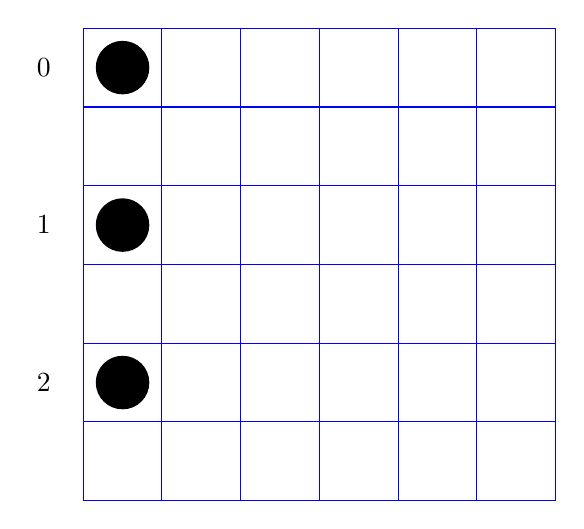
\begin{tikzpicture}[thick]
    \draw[blue, thin] (0,0) grid (6,6);
    \foreach \c in {(0,5),(0,3),(0,1)}
        \fill \c + (0.5,0.5) circle (0.34);
    \node at (-0.5,5.5) {$0$};
    \node at (-0.5,3.5) {$1$};
    \node at (-0.5,1.5) {$2$};
\end{tikzpicture}
\caption{Each dot corresponds  to a drone, while the grid is the field. This picture only shows a $6\times6$ grid, however in the simulation we envisioned a $30\times30$ one. }
\label{fig:grid}
\end{subfigure}\\

\begin{subfigure}{.5\textwidth}
  \centering
\begin{tabular}{|c|c|c|c|c|}

\hline
    Drone id & assigned area & corresponding images\\
\hline
    0& 1 & 0-179\\
    1& 2 & 180-359\\
    2& 3 & 360-539\\
    3& 4 & 540-719\\
    4& 5 & 720-899\\
\hline
\end{tabular}
\caption{Area assigned to each drone}
\label{tab:assigned_area}
\end{subfigure}

\caption{The simulation environment we visioned}
\label{fig:vision}
\end{figure}\\
Once the simulation is terminated, the output ought to be information about each cell of the grid, hence what type of plant the drone predicted in that cell. In order to obtain that, we  programmed the path each drone is supposed to take. Various suggestions have been considered, however, in order to represent a scenario as close as possible to a real world application, we settled for the strategy shown in Fig. n. \ref{fig:grid_path}. \\
In such scenario, the drones go back and forth in the assigned area 
keeping track of the plants (in this case, the images) it encounters saving the image and the prediction it makes. Fig. n. \ref{fig:grid_path} shows only the path which Drone 0 takes, however the other drones follow the same strategy to completely scan the entire assigned area. The result is then stored as a ''.csv'' file and the predictions are saved according to the order in which the drone encounters the pictures. For example, in case of Drone 0, the order is shown in Fig. n. \ref{fig:grid_path}. 
\begin{figure}
\centering
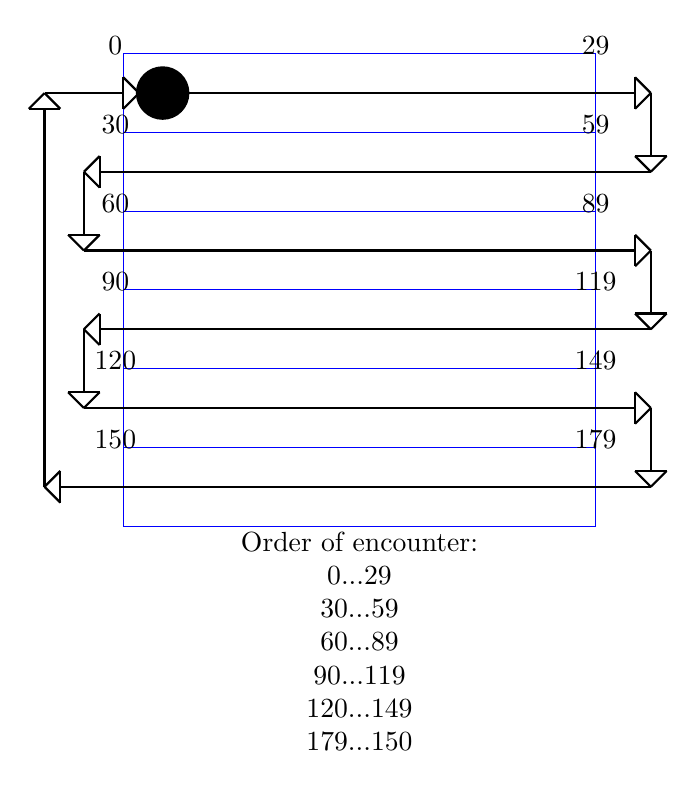
\begin{tikzpicture}[thick]
    \draw[blue, thin] (0,0) -- (0,6);
    \draw[blue, thin] (6,0) -- (6,6);
    \draw[blue, thin] (0,0) -- (6,0);
    \draw[blue, thin] (0,1) -- (6,1);
    \draw[blue, thin] (0,2) -- (6,2);
    \draw[blue, thin] (0,3) -- (6,3);
    \draw[blue, thin] (0,4) -- (6,4);
    \draw[blue, thin] (0,5) -- (6,5);
    \draw[blue, thin] (0,6) -- (6,6);
    \foreach \c in {(0,5)}
        \fill \c + (0.5,0.5) circle (0.34);
        %draw pictures numbers
    \node at (-0.1,6.1) {$0$};
    \node at (6,6.1) {$29$};
    \node at (-0.1,5.1) {$30$};
    \node at (6,5.1) {$59$};
    
    \node at (-0.1,4.1) {$60$};
    \node at (6,4.1) {$89$};
    \node at (-0.1,3.1) {$90$};
    \node at (6,3.1) {$119$};
    \node at (-0.1,2.1) {$120$};
    \node at (6,2.1) {$149$};
    \node at (-0.1,1.1) {$150$};
    \node at (6,1.1) {$179$};

        %%%%%%%%%%%%%%%%%%%%%%%%%%%%%%%%%%%
        %%%FirstPATH
        %%%%%%%%%%%%%%%%%%%%%%%%%%%%%%%%%%%
        %draw line left to right
    \draw  (0.5,5.5) -- (6.5,5.5);
        %draw triangle left to right
    \draw (6.5,5.7) -- (6.5,5.3);
    \draw (6.5,5.7) -- (6.7,5.5);
    \draw (6.7,5.5) -- (6.5,5.3);
        %draw line down to bottom 
    \draw  (6.7,5.5) -- (6.7,4.7);
        %draw triangle down to bottom 
    \draw  (6.5,4.7) -- (6.7,4.5);
    \draw  (6.9,4.7) -- (6.7,4.5);
    \draw (6.5,4.7) -- (6.9,4.7);
        %draw line right to left
    \draw  (6.7,4.5) -- (-0.3,4.5);
        %draw triangle right to left
    \draw  (-0.5,4.5) -- (-0.3,4.3);
    \draw  (-0.5,4.5) -- (-0.3,4.7);
    \draw  (-0.3,4.3) -- (-0.3,4.7);
        %draw line down to bottom (l)
    \draw  (-0.5,4.5) -- (-0.5,3.7);
        %draw triangle down to bottom (l)
    \draw  (-0.5,3.5) -- (-0.3,3.7);
    \draw  (-0.5,3.5) -- (-0.7,3.7);
    \draw  (-0.3,3.7) -- (-0.7,3.7);
        %%%%%%%%%%%%%%%%%%%%%%%%%%%%%%%%%%%
        %%%Second path
        %%%%%%%%%%%%%%%%%%%%%%%%%%%%%%%%%%%
        %draw line left to right
    \draw  (-0.5,3.5) -- (6.5,3.5);
        %draw triangle left to right
    \draw (6.5,3.7) -- (6.5,3.3);
    \draw (6.5,3.7) -- (6.7,3.5);
    \draw (6.7,3.5) -- (6.5,3.3);
        %draw line down to bottom 
    \draw  (6.7,3.5) -- (6.7,2.7);
        %draw triangle down to bottom 
    \draw  (6.5,2.7) -- (6.7,2.5);
    \draw  (6.9,2.7) -- (6.7,2.5);
    \draw (6.5,2.7) -- (6.9,2.7);
        %draw line right to left
    \draw  (6.7,2.5) -- (-0.3,2.5);
        %draw triangle right to left
    \draw  (-0.5,2.5) -- (-0.3,2.3);
    \draw  (-0.5,2.5) -- (-0.3,2.7);
    \draw  (-0.3,2.3) -- (-0.3,2.7);
        %draw line down to bottom (l)
    \draw  (-0.5,2.5) -- (-0.5,1.7);
        %draw triangle down to bottom (l)
    \draw  (-0.5,1.5) -- (-0.3,1.7);
    \draw  (-0.5,1.5) -- (-0.7,1.7);
    \draw  (-0.3,1.7) -- (-0.7,1.7);
    %%%%%%%%%%%%%%%%%%%%%%%%%%%%%%%%%%%
    %%%Third path
    %%%%%%%%%%%%%%%%%%%%%%%%%%%%%%%%%%%
        %draw line left to right
    \draw  (-0.5,1.5) -- (6.5,1.5);
        %draw triangle left to right
    \draw (6.5,1.7) -- (6.5,1.3);
    \draw (6.5,1.7) -- (6.7,1.5);
    \draw (6.7,1.5) -- (6.5,1.3);
        %draw line down to bottom 
    \draw  (6.7,1.5) -- (6.7,0.7);
        %draw triangle down to bottom 
    \draw  (6.5,0.7) -- (6.7,0.5);
    \draw  (6.9,0.7) -- (6.7,0.5);
    \draw (6.5,0.7) -- (6.9,0.7);
        %draw line right to left
    \draw  (6.7,0.5) -- (-0.8,0.5);
        %draw triangle right to left
    \draw  (-1,0.5) -- (-0.8,0.3);
    \draw  (-1,0.5) -- (-0.8,0.7);
    \draw  (-0.8,0.3) -- (-0.8,0.7);
        %draw line upwards
    \draw  (-1,0.5) -- (-1, 5.3);
        %draw triangle upwards
    \draw  (-1,5.5) -- (-1.2, 5.3); 
    \draw  (-1,5.5) -- (-0.8, 5.3); 
    \draw  (-1.2, 5.3) -- (-0.8, 5.3); 
        %draw line left to right
     \draw  (-1,5.5) -- (0, 5.5);  
        %draw triangle left to right
    \draw (0.2,5.5) -- (0, 5.7);
    \draw (0.2,5.5) -- (0, 5.3);
    \draw (0, 5.7) -- (0, 5.3);
      
    \node at (3,-1.5) {\begin{tabular}{c}
    Order of encounter:\\
    0...29\\
    30...59\\
    60...89\\
    90...119\\
    120...149\\
    179...150\\
    \end{tabular}};
       
\end{tikzpicture}
\caption{Example of the drones' path. In this picture, only the path taken by Drone 0 is represented, however, following Fig. n. \ref{tab:assigned_area}, it is trivial to figure out the path of the other drones as well. }
\label{fig:grid_path}
\end{figure}

\newpage
\section{Conclusion}
In this paper we explored our vision for an automated farming system which can improve the working life of many farmers. With the use of cheap and wide available technology we are able to develop a fully automated system which is able to replace the most time-consuming tasks and help the farmers focus on other duties. \\
We first started from analysing the main requirements to fulfill in order to achieve such ambitious goal. Moreover, we identified the entities required to act and more importantly the actions they need to make in order to not only create a functional and practical system, but also to insure safety and preserve the quality of the product. \\
Subsequently, we utilized TAPAAL to model the behaviour of the aforementioned entities and to verify that the most important properties were satisfied. We used this models as as the foundation for our simulation, because, by following them, it is safe to assume that our system would be correct and safe. \\
Finally, we discussed our simulation. We defined each step that took us to the development of an application that could give us an idea of how our system would perform in a real world application. Since we simulated drones able to recognize plants, we collected an appropriate data-set to replicate a field with different vegetation on it. We trained a Deep Neural Network able to recognize those plants with high efficiency and we defined a routine for the drones to follow to efficiently scan the field. \\
The result of our exploration is an efficient, cheap and practical system that can be applied to most of the plantation to increment production and yield quality. The results are very promising and, based on those, we are confident that in the future our application will be a reality and that it will help improving the working life of the workers.

\newpage
\bibliography{mybibfile}
\newpage
\section{Appendix}\label{sec:appendix}
\begin{figure}[H]
    \centering
    \includegraphics[width = 12cm]{img/sentinel.png}
    \caption{TAPAAL model of the sentinel.}
    \label{fig:sentinel}
\end{figure}
\begin{figure}
    \includegraphics[width = 12.6cm]{img/datasetfig2.jpg}
    \caption{Example for each of the class contained in the data-set. All the classes are in the table below: \\
    \centerline{
    \begin{tabular}{c|c|c}
         black grass&charlock&cleavers \\
         common chickweed&common wheat&fat hen \\
         loose silky bent&maize&scentless mayweed\\
         shepherds purse&small flowered cranesbill&sugar beet\\
    \end{tabular}}
    }
    \label{fig:datasetfig2}
\end{figure}

\newpage
\section{Declaration of Originality}
We,
\begin{itemize}
    \item[] Luca Brodo
    \item[] Niklas Kohlhage
    \item[] Carl-Georg Meyer
    \item[] Jonas Weißbrod
\end{itemize}

herewith declare that we have composed the present paper by ourselves and without use of any other than the cited sources and aids. Sentences or parts of sentences quoted literally are marked as such; other references with regard to the statement and scope are indicated by full details of the publications concerned. The paper in the same or similar form has not been submitted to any examination body and has not been published. This paper was not yet, even in part, used in another examination or as a course performance. We consent to have our work checked with a plagiarism checker if deemed necessary.

Hamm/Lippstadt, January 14\textsuperscript{th}, 2022

This certificate is valid without signatures of the named individuals. Handwritten changes are only valid if they are officially confirmed by at least one of the named individuals.
\end{document}